\lab{Электромагнитные волны в волноводе}
\todo[author=Tiffani]{Номер лабораторной?}
\todo[author=Tiffani]{Необходимо сделать рисунки во всю лабораторную}
\begin{lab:aim}
ознакомление с особенностями распространения электромагнитных волн в волноводе, аппаратурой и методами измерения основных характеристик протекающих при этом процессов.
\end{lab:aim}

\begin{lab:equipment}
генератор сигналов сверхвысокой частоты, измерительная линия, усилитель, заглушка, отрезок волновода с поглощающей нагрузкой, отрезки волноводов различных сечений, детекторная головка.
\end{lab:equipment}

Передача энергии электромагнитных колебаний низкой частоты, например, 50~Гц, не представляет проблем и делается широко известным способом: по проводам. На более высоких частотах (до 300~МГц) эта задача решается с помощью двухпроводных линий и коаксиальных кабелей. На ещё более высоких частотах (до 300~ГГц) при колебаниях с длинами волн (в вакууме) от 1~метра до 1~миллиметра (этот диапазон называется \important{диапазоном сверхвысоких частот} или, сокращённо, СВЧ) передача энергии с помощью двухпроводной линии или коаксиальных кабелей становится малоэффективной из-за больших потерь: резко возрастает сопротивление проводов из-за \important{скин-эффекта}~---~вытеснения тока на поверхность, а в двухпроводной линии, кроме того, потери растут вследствие излучения энергии в окружающее пространство.

В СВЧ-диапазоне энергия передаётся с помощью металлических труб, называемых волноводами (в миллиметровом диапазоне длин волн волноводы могут быть сделаны и из диэлектрика). Электромагнитные волны могут распространяться по металлическим трубам любого профиля, но из технологических соображений сечения волноводов делаются либо круглыми, либо прямоугольными.

Чтобы найти структуру электромагнитного поля в волноводе, надо решить уравнения Максвелла с соответствующими граничными условиями. Решение этой задачи приведено во многих учебниках.

Для радиоволн, бегущих по волноводу вдоль оси $Z$ с проводящими стенками, расположенными на расстоянии $a$ друг от друга (простейший волновод), с вектором напряженности электрического поля $\vec E=E_y \vec e_y,$ перпендикулярным плоскости $ZX$. Такое решение может быть записано в виде:
\begin{equation}
	\eqmark{2.0.1}
	E_y=A\sin\left(\dfrac{n\pi x}{a}\right)\sin(\omega t-k_zz), \qquad n=0,~1,~2,~3 \ldots,
\end{equation}
где $k_z=\sqrt{k^2-k^2_x}, k=2\pi/\lambda_0=\omega/c, \lambda_0$~---~длина волны в вакууме, $\omega=2\pi f$, $f$~---~частота генератора, $c$~---~скорость света. Множитель $\sin\left(\dfrac{n\pi x}{a}\right)$ физически соответствует стоячей волне между стенками волновода по координате $Х$ и определяет граничные условия $E_y=0$ на проводящих стенках.
	
\begin{figure}[h!]
	%\centering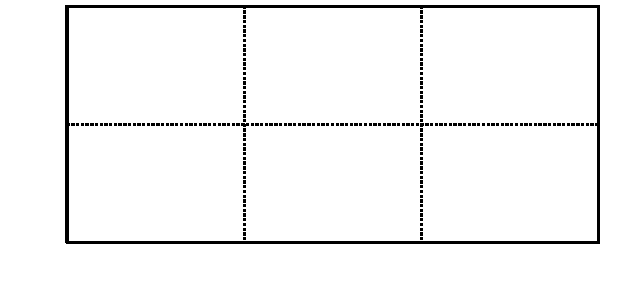
\includegraphics[width=0.6\linewidth]{Chapter_2/13}
	\caption{Волновод и примеры распределения поля}
	\figmark{waveguide}
\end{figure}
	
Для бегущих вдоль волновода волн $k_z$~---~действительная величина. Предельный случай $k_z=0$ соответствует $k=k_x,$ что при условии $n=1$ приводит к формулам для \important{критических длины и циклической частоты волн}, распространяющихся в вакуумном волноводе:
\begin{equation}
	\eqmark{2.0.2}
	\lambda_{\text{кр}}=2a, \qquad \omega_{\text{кр}}=\pi c/a.
\end{equation}
Если $\lambda>2a$ и, соответственно, $\omega<\pi c/a,$ то электромагнитная волна при распространении вдоль волновода затухает.

Для бегущей волны фазовая скорость 
\begin{equation}
	\eqmark{2.0.3}
	V_{\text{Ф}}=\omega/k_z=c/\sqrt{1-\omega^2_{\text{кр}}/\omega^2}
\end{equation}
больше скорости света в вакууме $c,$ а длина волны в волноводе
\begin{equation}
	\eqmark{2.0.4}
	\lambda_{\text{В}}=\lambda_0/\sqrt{1-(\lambda_0/2a)^2}
\end{equation}
больше длины волны в вакууме $\lambda_0.$
В представленном на рис.~\figref{waveguide} случае отлична от нуля продольная составляющая магнитного поля, и такую волну называют \important{магнитной ($H$-волна).} Обычно для передачи СВЧ-энергии по прямоугольному волноводу используется волна (мода) $H_{10}.$  Второй индекс $0$ соответствует отсутствию составляющей электромагнитного поля $E_x.$ Критическая длина волны моды $H_{10}$~---~максимальная среди всех типов волн в прямоугольном волноводе, и поэтому ее называют \important{основной.} Тем самым, для волновода заданного сечения существует диапазон частот, ограниченный снизу критической частотой волны $H_{10}$ ($\lambda_{\text{кр}}=2a$). Следующая по возрастанию частоты~---~мода $H_{01}$ с $\lambda_{\text{кр}}=2b$ или $H_{20}$ с $\lambda_{\text{кр}}=a,$ если $a>b.$

В заданном частотном диапазоне СВЧ-энергия может переноситься одним типом волн, что существенно облегчает её дальнейшее использование.

Если в волноводе имеется какое-либо препятствие, нерегулярность, то в нём появляется \important{отражённая волна.} Падающая $E_0$ и отраженная волна с коэффициентом отражения $\rho$ по амплитуде интерферируют и создают в волноводе стоячую волну.

Максимальное (в пучности) и минимальное (в узле) значения поля равны соответственно
\begin{equation}
	\eqmark{2.0.5}
	E_{\text{max}}=E_0(1+\rho), \qquad E_{\text{min}}=E_0(1-\rho).
\end{equation}
Отношение $K=E_{\text{max}}/E_{\text{min}}$ называется \important{коэффициентом стоячей волны} (к.с.в.). Коэффициент отражения от препятствия по амплитуде
\begin{equation}
	\eqmark{2.0.6}
	\rho=\dfrac{E_{\text{max}}-E_{\text{min}}}{E_{\text{max}}+E_{\text{min}}}=\dfrac{K-1}{K+1}.
\end{equation}

В случае полного отражения (металлическая заглушка) $\rho=1,$ а если в волновод вставлено вещество, поглощающее СВЧ-­излучение (согласованная нагрузка), то $\rho=0.$

Для определения коэффициента стоячей волны обычно используют измерительную линию~---~отрезок волновода с продольной щелью длиной в несколько полуволн. В щели располагается зонд~---~большой металлический штырь (антенна), реагирующий на электрическое поле в волноводе. Напряжение высокой частоты, наводимое на зонд, детектируется, усиливается и подаётся на микровольтметр. Зонд может перемещаться вдоль линии, что позволяет исследовать распределение электрического поля в волноводе.

\labsection{А. Волны в волноводе при частоте выше критической}

\experiment
Схема для исследования структуры волн в волноводе при частоте выше критической представлена на рис.~\figref{scheme microwave}. Модулированный сигнал от высокочастотного генератора (цуги с частотой повторения 1~кГц) поступает на вход измерительной линии, вдоль которой перемешается зонд~8. Высокочастотный сигнал с зонда поступает на кристаллический детектор $D$.

\begin{figure}[h!]
	%\centering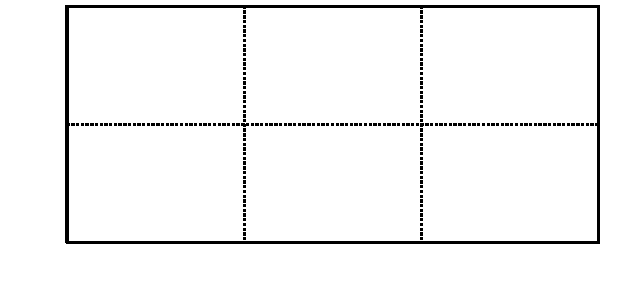
\includegraphics[width=0.6\linewidth]{Chapter_2/13}
	\caption{Схема для исследования структуры волн СВЧ}
	\figmark{scheme microwave}
\end{figure}

С нагрузки детектора (с $RС$-цепочки) снимается огибающая высокочастотного сигнала и подаётся на усилитель низкой частоты. Величина сигнала регистрируется вольтметром, вмонтированным в усилитель. Ручка~$С$~---~настройка измерительной линии~--- служит для согласования зонда (как антенны) со входом усилителя. Как правило, они согласованы, и в настройке нет необходимости. В волноводе с закрытым выходом образуется стоячая волна. Определив расстояние между узлами, можно рассчитать длину волны и фазовую скорость СВЧ-сигнала в волноводе. Устройство детекторной головки, установленной на измерительной линии, таково, что отклик вольтметра $U$ на величину напряжённости электрического поля $Е$ в волноводе 
\begin{equation*}
	U\sim E^{n},
\end{equation*}
а показатель степени $n$ сам зависит от величины сигнала: при малых сигналах детектирование квадратичное $(n=2),$ при больших~---~линейное $(n=1).$

Меняя нагрузку на выходе измерительной линии (ручка~$B$ на рис.~\figref{scheme microwave}) и сравнивая максимальное и минимальное показания вольтметра, можно рассчитать коэффициент стоячей волны $K$ и коэффициент отражения $\rho.$

\labsection{Б. Волны в волноводе при частоте ниже критической}

Для исследования затухания волн в волноводе при частоте ниже критической используются те же генератор, усилитель, измерительная линия и дополнительный набор волноводов с отдельной детекторной головкой $G$ (рис.~\figref{scheme damping}). Дополнительный набор начинается и заканчивается волноводами переменного сечения I и II. Между ними

\begin{figure}[h!]
	%\centering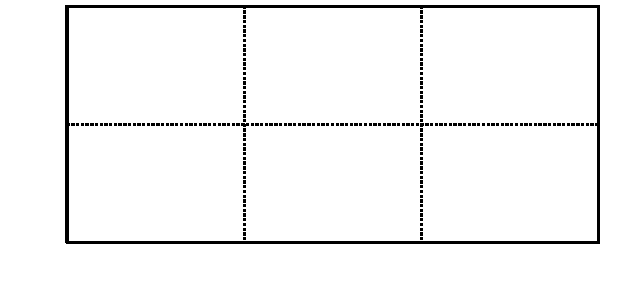
\includegraphics[width=0.6\linewidth]{Chapter_2/13}
	\caption{Схема для исследования затухания}
	\figmark{scheme damping}
\end{figure}

можно разместить 1,~2 или 3 одинаковых отрезка с постоянным сечением. В такой системе волны с частотами меньше критической экспоненциально затухают.

Мощность сигнала на выходе из волновода $W$ можно связать с мощностью входного сигнала $W_0$ двумя способами: $W=W_0e^{-\alpha z}$ или $W=W_0~10^{-\beta z},$ где $z$~---~длина волновода. Величина $(\alpha z)$ измеряется в Неперах (Нп): один Непер соответствует отношению интенсивностей, равному основанию натуральных логарифмов. Величину $(\beta z)$ принято измерять в децибелах (дБ): один Бел соответствует уменьшению мощности в 10 раз; децибел~---~одна десятая Бела. Измеренное в децибелах затухание определяется формулой $\beta z(\text{дБ})=10\times\lg(W_0/W).$ Отсюда следует, что $\alpha(\text{Нп})=2,3\beta(\text{Б}).$

Если при уменьшении количества вставок волновода поддерживать интенсивность выходного сигнала постоянной, то входной сигнал следует ослабить. Степень ослабления $\gamma$ зависит от длины волновода $z~(\gamma~=~\beta~z)$ и измеряется по шкале генератора в децибелах. Именно таким образом в эксперименте определяется коэффициент затухания $\beta.$ Его можно сравнить с коэффициентом $\alpha,$ рассчитанным теоретически. В закритическом волноводе при квадратичном детектировании интенсивность сигнала падает по закону $E^2\sim e^{-\alpha z},$ где $\alpha$~---~коэффициент затухания:
\begin{equation}
	\eqmark{2.0.7}
	\alpha=2ik_{Z}=\dfrac{2\omega}{c}\sqrt{\left(\dfrac{\omega_{kp}}{\omega}\right)^2-1}=\dfrac{2\pi}{a}\sqrt{1-\left(\dfrac{2a}{\lambda_0}\right)^2}.
\end{equation}
Здесь $\lambda_0=c/f=3,22$~см – длина волны в свободном пространстве, соответствующая рабочей частоте $f=9320$~МГц, $a=1,6$~см~---~размер широкой стенки волновода-вставки.

\begin{lab:task}

В работе предлагается при частоте выше критической исследовать стоячую волну в измерительной линии (рис.~\figref{scheme microwave}): измерив распределение сигнала вдоль волновода, рассчитать фазовую скорость; затем, меняя нагрузку на выходе волновода (заглушка, открытый конец или поглотитель), определить коэффициенты отражения волн $\rho.$ При частоте ниже критической предлагается определить коэффициент затухания волны $\beta$ в сборном волноводе (рис.~\figref{scheme damping}) и сравнить с его теоретическим значением.

	\tasksection{А. Исследование структуры волн при частоте выше 
		критической}

Мощность сигнала, снимаемого с генератора Г4-83, невелика, поэтому излучение не представляет опасности для здоровья человека. Тем не менее, заглядывать в открытый волновод при включённом генераторе не рекомендуется.

\begin{enumerate}
	\tasksection{I. Определение длины волны СВЧ-сигнала в волноводе}

	\item Проведите подготовку приборов к работе по техническому описанию (ТО), лежащему на рабочем столе.
	
	\item Установите рабочую частоту $f=9320$~МГц; перемещая зонд, настройтесь на пучность стоячей волны. Если при этом показания вольтметра превышают 1~мВ, следует ослабить сигнал, идущий от генератора, с помощью аттенюатора~4 (при напряжениях $\ge1$~мВ меняется характер детектирования).
	
	\item С помощью переключателей~5 и 9 подберите чувствительность вольтметра так, чтобы в максимуме стрелка отклонялась почти на всю шкалу. Используя весь возможный диапазон перемещения зонда вдоль измерительной линии, снимите зависимость показаний вольтметра $U$ от положения зонда $z$ (100 делений винта у выхода измерительной линии соответствуют 1~мм). Менять чувствительность вольтметра в течение этой серии нецелесообразно.
	
	\item Постройте график $U(z)$ и определите по нему длину волны $\lambda_{\text{В}}$ в волноводе. Сравните результат с теоретическим расчётом. Рассчитайте фазовую скорость $V_{\text{Ф}}$ волн в волноводе по формуле \eqref{2.0.3}. Рассчитайте групповую скорость $u,$ используя соотношение $uV_{\text{Ф}}=c^2.$	

	\tasksection{II. Определение коэффициентов отражения}

    \item Снимите металлическую заглушку с фланца измерительной линии. Перемещая зонд, измерьте максимальное ($U_{\text{max}}<1$~мВ) и минимальное напряжения в волне.
    
   \item Наденьте на выходной фланец измерительной линии отрезок волновода с поглощающей нагрузкой и снова измерьте максимальное и минимальное напряжения.
   
   \item Считая детектирование квадратичным, определите коэффициенты отражения $\rho$ для открытого и закрытого волновода и для волновода с поглощающей нагрузкой. Объясните полученные результаты. 

\tasksection{Б. Исследование затухания волн при частоте ниже
  		критической}
   
	\item Соберите схему согласно рис.~\figref{scheme damping} и настройте её по техническому описанию (ТО).
  
  \item Измерьте длину каждой волноводной секции.
  
  \item Рассчитайте критическую частоту для этого волновода ($f_{\text{кр}}=c/2a$, $a=1,6$~см) и убедитесь, что рабочая частота $f=9320$~МГц меньше критической.

	\tasksection{III. Измерение коэффициента затухания}

   \item Настройте детекторную головку на максимальную чувствительность согласно ТО, расположенному на установке (в этом упражнении ограничение $U<1$~мВ необязательно). Установите минимальное затухание ($\gamma=20$~дБ) сигнала от генератора и подберите чувствительность вольтметра так, чтобы стрелка отклонялась почти на всю шкалу; зарегистрируйте величины $U$ и $\gamma.$
   
   \item Последовательно уменьшая число промежуточных секций от трёх до нуля, каждый раз подбирайте такое ослабление сигнала от генератора, при котором показания вольтметра усилителя остаются неизменными.
   
  \item Постройте график в функции $\gamma=f(z),$ где $z$~---~полная длина подключенных волноводных секций. По наклону прямой рассчитайте коэффициент затухания $\beta=\Delta\gamma/\Delta z$ в единицах $\text{Б}/\text{см}$ и сравните с таким же коэффициентом, рассчитанным теоретически.
	\end{enumerate}
\end{lab:task}

\begin{lab:questions}

	\item Используя выражения для фазовой и групповой скоростей: $V_{\text{Ф}}=\omega/k$, $u=d\omega/dk,$~--- покажите, что в волноводе выполняется соотношение $uV_{\text{Ф}}=c^2.$
	
	\item Как направлен вектор Пойнтинга в волноводе?
\end{lab:questions}

\begin{lab:literature}

	\item \emph{Сивухин~Д.В.} Общий курс физики. – Т.~III, Электричество. – М.:~Физматлит, 2006, §§~139,~140.
	
	\item \emph{Кингсепп~А.С., Локшин~Г.Р., Ольхов~О.А.} Основы физики. Т.~1. – М.:~Физматлит, 2001, §~6.7.
	
	\item Фейнмановские лекции по физике. Т.~6. Электродинамика. – М.:~Наука, 1966, гл.~24.
	
\end{lab:literature}